
\documentclass[12pt]{article}
\usepackage{amsmath}
\DeclareMathOperator*{\argmin}{arg\,min} % thin space, limits underneath in displays
\DeclareMathOperator*{\argmax}{arg\,max} % thin space, limits underneath in displays
\newtheorem{thm}{Theorem}
\usepackage{amssymb}
\usepackage{amsfonts}
\usepackage{mathrsfs}
\usepackage{bm}
\usepackage{indentfirst}
\setlength{\parindent}{0em}
\usepackage[margin=1in]{geometry}
\usepackage{graphicx}
\usepackage{setspace}
\doublespacing
\usepackage[flushleft]{threeparttable}
\usepackage{booktabs,caption}
\usepackage{float}
\usepackage{graphicx}
\usepackage[sort,comma]{natbib}
\usepackage[hidelinks]{hyperref}

\usepackage{import}
\usepackage{xifthen}
\usepackage{pdfpages}
\usepackage{transparent}

\newcommand{\incfig}[1]{%
\def\svgwidth{\columnwidth}
\import{./figures/}{#1.pdf_tex}
}




\title{Exogenous Nominal Rigidity}
\author{}
\date{}


\begin{document}
\maketitle

A Walrasian model that is, a competitive model without any externalities,
asymmetric information, missing markets, or other imperfections.

\section{A baseline Case: Fixed Prices}
We assume the nominal price is fixed.

\subsection{Assumptions}
1. Time is discrete. Labor is the only input.
\begin{equation*}
F = F(L), \quad F'(\cdot ) > 0, \quad F''(\cdot ) \le 0
\end{equation*}

2. HHs obtain utility from 1) consumption, 2)holding real money balance, and disutility
from 3) working.
The HH's objective function,
\begin{equation*}
{\rm I\!{U}} = \sum\limits_{t = 0} ^\infty \beta^{t}	\left[ 
		U(C_{t}) + \Gamma \left( \frac{M_{t}}{P_{t}} \right)  - V(L_{t})
\right] , \quad \beta \in (0,1)
\end{equation*}
\begin{equation*}
U' > 0, U'' < 0, \Gamma' > 0, \Gamma '' < 0, V'>0, V'' < 0
\end{equation*}
$ U $ and $ \Gamma $ are in constant-relative-risk-aversion forms:
\begin{align*}
U(C_{t}) &= \frac{C_{t}^{1 - \theta}}{1 - \theta}, \quad \theta > 0\\
\Gamma \left( \frac{M_{t}}{P_{t}} \right)  &=
\frac{\left( \frac{M_{t}}{P_{t}} \right) ^{1 - \chi}}{1 - \chi}, \quad \chi > 0
\end{align*}

HHs obtain positive utility from holding cash because it allows them to purchase some
goods more easily.


3. Two assets:\\
1) Money, pays interest rate of 0.\\
2) Bond, pays interest rate of $ i_{t} $.

\begin{align*}
A_{t}&: \text{ HH's wealth at the start of period $ t $. }\\
W_{t}L_{t}&: \text{ labor income }\\
W_{t}&: \text{ nominal wage }\\
P_{t}C_{t}&: \text{ consumption expenditures }\\
M_{t}&: \text{ money in hand }
\end{align*}
HH spends the rest of income buying bonds. Hence, the bond it can hold from $ t $
to $ t + 1 $ is
\begin{equation*}
A_{t} + W_{t}L_{t} - P_{t}C_{t} - M_{t}
\end{equation*}

Therefore, the accumulation of wealth is
\begin{align*}
A_{t + 1} &= M_{t} + \text{ bonds and interest payment bring to $ t + 1 $ }\\
A_{t + 1}&= M_{t} + (A_{t} + W_{t}L_{t} - P_{t}C_{t} - M_{t})(1 + i_{t})
\end{align*}
HH takes $ W, P, i $ as give. It chooses $ C $ and $ M $ to maximize the utility.

The path of $ M $ is set by the central bank. Thus, although HHs view the path of $ M $
as something they choose, in general equilibrium, the path of $ M $ is exogenous,
and the path of $ i $ is determined endogenously.


\subsection{Utility maximization}
Rewrite asset accumulation process,
\begin{align*}
{\rm I\!{U}} &= \sum\limits_{t = 0} ^\infty \beta^{t}	\left[ 
		U(C_{t}) + \Gamma \left( \frac{M_{t}}{P_{t}} \right)  - V(L_{t})
\right] \\
A_{t + 1}&= M_{t} + (A_{t} + W_{t}L_{t} - P_{t}C_{t} - M_{t})(1 + i_{t})\\
C_{t}&= \left[ A_{t} + W_{t}L_{t} - M_{t} - \frac{A_{t + 1} - M_{t}}{1 + i_{t}} \right] 
\frac{1}{P_{t}}\\
		 &= a_{t} + w_{t}L_{t} - \frac{i_{t}m_{t}}{1 + i_{t}} - \frac{a_{t + 1}}{1 + r_{t}}
\end{align*}

Plug in $ C_{t} $ into the lifetime utility function and differentiate it wrt 
$ A_{t + 1} $ to obtain the FOC.
\begin{align*}
\frac{\partial U }{\partial A_{t + 1} }&= 
\beta^{t}U'(C_{t})\left[ \frac{1}{P_{t}}\left(  - \frac{1}{1 + i_{t}} \right)  \right] 
 + \beta^{t + 1}U'(C_{t + 1})\frac{1}{P_{t + 1}} = 0\\
 U'(C_{t})\frac{1}{P_{t}}\frac{1}{1 + i_{t}} &= \beta U'(C_{t + 1})\frac{1}{P_{t + 1}}\\
 U'(C_{t})\frac{P_{t + 1}}{P_{t}}\frac{1}{1 + i_{t}}&= \beta U'(C_{t + 1}), \quad
 1 + \pi_{t} = \frac{P_{t + 1}}{P_{t}}\\
 U'(C_{t})\frac{1 + \pi_{t}}{1 + i_{t}}&= \beta U'(C_{t + 1}), \quad
 (1 + i_{t}) = (1 + r_{t})(1 + \pi_{t})\\
 U'(C_{t}) &= \beta(1 + r_{t})U'(C_{t + 1})\\
 C_{t}^{ - \theta}&= \beta(1 + r_{t})C_{t + 1}^{ - \theta}
\end{align*}

Take log
\begin{equation*}
\ln C_{t} = \ln C_{t + 1} - \frac{1}{\theta}\ln (1 + r_{t})\beta
\end{equation*}

Let's make some changes to this equation. Recall that the only use of output is for
consumption. And we normalize the number of HHs to 1. Then we can replace $ C $ by
$ Y $. In addition, because for small values of $ r $, $ \ln (1 + r)\approx r $. 
Replace $ \ln (1 + r) $ by $ r $. We receive this:
\begin{equation}
		\label{eqn:new keynesian IS}
\ln Y_{t} = a + \ln Y_{t + 1} - \frac{1}{\theta}r_{t}
\end{equation}
where $ a =  - \frac{1}{\theta}\ln \beta $.

Equation \eqref{eqn:new keynesian IS} is called {\textbf {the New Keynesian IS curve.}}


\noindent\fbox{%
\parbox{\textwidth}{%
{\textbf {New vs. Traditional Keynesian IS curve}}

They are different on the RHS,  the presence of $ Y_{t + 1} $.

Traditional Keynesian IS curve does not have $ Y_{t + 1} $:
\begin{equation}
\ln Y_{t} = a - \frac{1}{\theta}r_{t}
\end{equation}

Traditional IS is based on the idea that an increase in $ r $ reduces $ I $. Consumption
is completely unresponsive to the real interest rate.

New IS is derived from a model where $ I $ (investment) is absent. And the response
of consumption to the real interest rate is central to the equation.

}%
}\\


Rewrite the asset accumulation process in real terms
\begin{align*}
C_{t}&= \left[ A_{t} + W_{t}L_{t} - M_{t} - \frac{A_{t + 1} - M_{t}}{1 + i_{t}} \right] 
\frac{1}{P_{t}}\\
&= a_{t} + w_{t}L_{t} - \frac{i_{t}m_{t}}{1 + i_{t}} - \frac{a_{t + 1}}{1 + r_{t}}
\end{align*}
Find how money affect consumption
\begin{align*}
\frac{\partial C_{t} }{\partial m_{t} } =  - \frac{i_{t}}{1 + i_{t}}
\end{align*}


Solve FOC for $ m_{t} $:
\begin{align*}
{\rm I\!{U}} &= \sum\limits_{t = 0} ^\infty \beta^{t}	\left[ 
		U(C_{t}) + \Gamma \left( \frac{M_{t}}{P_{t}} \right)  - V(L_{t})
\right] \\
C_{t}&= a_{t} + w_{t}L_{t} - \frac{i_{t}m_{t}}{1 + i_{t}} - \frac{a_{t + 1}}{1 + r_{t}}
\\
\frac{\partial U }{\partial m_{t} }&= \Gamma'(m_{t}) - \frac{i_{t}}{1 + i_{t}}U'(C_{t})
=0\\
\Gamma'(m_{t})&= \frac{i_{t}}{1 + i_{t}}U'(C_{t})
\end{align*}
Plug in the Utility for $ C $ and $ \frac{M}{P} $, and using $ Y_{t} = C_{t} $
\begin{equation}
		\label{eqn:lm}
\left( \frac{M_{t}}{P_{t}} \right)^{d}  = 
m_{t} = Y_{t}^{\frac{\theta}{\chi}}\left( \frac{1 + i_{t}}{i_{t}} \right)^{
\frac{1}{\chi}}
\end{equation}
Money demand is positively correlated with output, and negatively correlated with
the nominal interest rate because $ i_{t} $ is a cost of holding money.

If we rewrite equation \eqref{eqn:lm},
\begin{equation*}
Y_{t} = m_{t}^{\frac{\chi}{\theta}}\left( \frac{1}{\frac{1}{i_{t}} + 1} \right) 
^{\frac{1}{\theta}}
\end{equation*}
You will find $ Y_{t} $ and $ i_{t} $ are positively correlated. This is the 
{\textbf {LM}} curve.

Now we have {\textbf {IS and LM curve}} (Investment-Saving, Liquidity-Money)
\begin{align*}
IS&:
\ln Y_{t} = a + \ln Y_{t + 1} - \frac{1}{\theta}r_{t}\\
LM &:
Y_{t} = m_{t}^{\frac{\chi}{\theta}}\left( \frac{1}{\frac{1}{i_{t}} + 1} \right) 
^{\frac{1}{\theta}}
\end{align*}

\begin{figure}[H]
\center{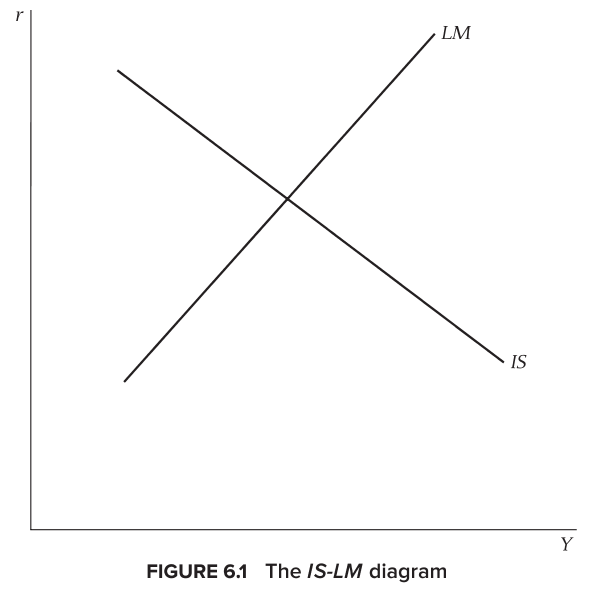
\includegraphics[scale =.5 ]  {figures/IS-LM.png}}
\end{figure}

{\textbf {Nominal Rigidity:}}
Now we fixed the price $ P_{t} =  \overline{P} $, an increase in the money supply,
$ M_{t} $, will increase the real money, $ m_{t} $, then the LM curve shift to the 
right. $ r_{t} $ goes down, $ Y_{t} $ goes up.

It says that with nominal rigidity, monetary disturbances have real effect.



\section{Price Rigidity, Wage Rigidity, and imperfections}
We will introduce four cases, the first two are baselines, but appear to fail
in describing the actual economies. The other two are more complicated and potentially
more accurate.
\subsection{Case 1: Keynes's Model}
The supply side: 

1. The nominal wage, $ W $, is completely unresponsive to current period developments.
\begin{equation*}
W =  \overline{W}.
\end{equation*}

2. The labor market has some non-Walrasian feature that causes the equilibrium real
wage, $ w_{t} $, to be above the market-clearing level.

Price $ P $ is flexible, and firms pay labor at MPL
\begin{equation*}
F'(L) = \frac{W}{P}
\end{equation*}
We start at point $ E $. For some reasons, there's an increase in aggregate demand
(demand for the product),
which leads to an rise in the price level, and lower the real wage, $ w $. And firms
hire more people. 
This view of the supply side of the economy implies a countercyclical real wage in 
response to aggregate demand shocks (an increase in demand reduces the real wage).

\begin{figure}[H]
\center{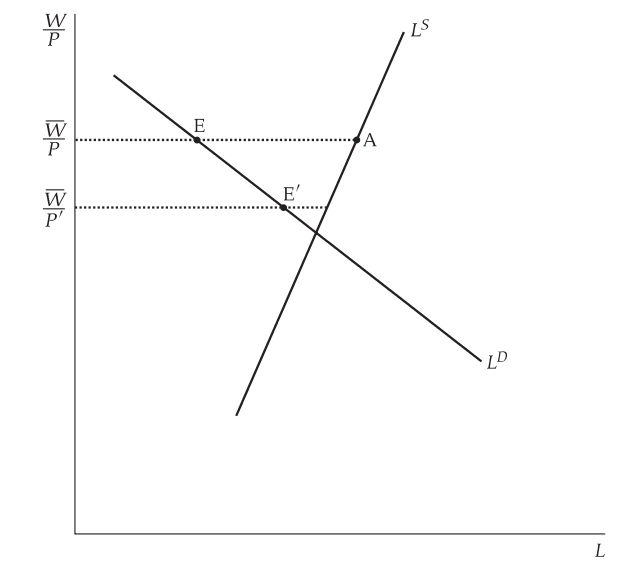
\includegraphics[scale =.5 ]  {figures/keynes's_sticky_wage.png}}
\end{figure}




\subsection{Case 2: Sticky prices, flexible wages, and a competitive labor mkt}
We discussed model of nominal rigidity in labor market.

Models of nominal rigidity in the goods market usually assume that firms have monopoly
power to sell the price above the MC. Hence, firms are better off if they can sell more
at the prevailing price. As a result, a rise in demand with rigid prices leads to
higher output.

When prices rather than wages are assumed rigid, $ P =  \overline{P} $.

From the FOC for $ L_{t} $:
\begin{align*}
U'(C_{t})w_{t} &= V'(L_{t})\\
C^{ - \theta}w_{t}&= V'(L_{t})\\
F(L_{t})^{ - \theta}w_{t}&= V'(L_{t}), \quad C = Y = F(L) \text{ at equilibrium }\\
w_{t}&= F(L_{t})^{\theta}V'(L_{t})
\end{align*}
where $ w_{t} $ stands for the real wage rate, $ \frac{W_{t}}{P_{t}} $.

It says $ L_{t} $ is positively correlated with $ w_{t} $.
\begin{equation*}
L = L^{s}\left( \frac{W}{P} \right) , \quad L^{s}(\cdot )' > 0
\end{equation*}




\section{Empirical application}
Various authors have examined the cyclical behavior of real wages using panel data.
DataSource: Panel Study of Income Dynamics (PSID).

Solon, Barsky, and Parker (1994) described that the aggregate real wage is unusually
procyclical from 1967-1987

They estimate
\begin{equation*}
\Delta \ln w_{it} = a'X_{it} + b \Delta u_{t} + e_{it}
\end{equation*}
individual $ i $, year $ t $, real wage $ w $, unemployment rate $ u $, vector of 
control variables $ X $.

Their result shows that a fall in the unemployment rate of 1\% is associated with a rise
in a typical worker's real wage of about 1.2 \% (statistically significant).


\section{Toward a usable model with exogenous nominal rigidity}
\subsection{A permanent output-inflation trade-off}
In previous sections, we assume that prices, wages, and money supply are fixed.
This is not realistic. These are not useful for addressing more practical questions.

We need to relax these assumptions.

For example, in Keynes's model, we assume nominal wage is fixed while price is flexible.
Now let's assume that the nominal wage rate, $ W_{t} $ is proportional to the previous
price level.
{\textbf {Hence, wages are adjusted for previous period's inflation.}}
\begin{equation*}
W_{t} = AP_{t - 1},\quad A > 0
\end{equation*}
Since employment is determined by $ MPL = w $, 
\begin{align*}
F'(L_{t})&= \frac{W_{t}}{P_{t}}\\
&= \frac{AP_{t - 1}}{P_{t}}\\
&= \frac{A}{1 + \pi_{t}}
\end{align*}
It says inflation and employment $ L $ are positively correlated.
{\textbf {It implies a permanent output-inflation trade-off:}} by accepting higher 
inflation, policymakers can permanently raise output.


Phillips (1958) showed that there was a {\textbf {strong  and relatively stable 
negative relationship between unemployment and wage inflation.}}
It is known as the Phillips curve.


\subsection{The Expectations-Augmented Phillips Curve}
Modern non-micro-founded formulations of pricing behavior differ from the simple
models in the previous section in three ways:

1. Prices and wages are flexible and are respond to the current state of the economy.

2. Allow supply shocks.

3. Adjustment to past and expected future inflation is assumed to be more complicated.

An example:
\begin{equation}
\label{eqn:augmented PHILLIPS}
\pi_{t} = \pi_{t}^{*} + \lambda(\ln Y_{t} - \ln  \overline{Y}_{t}) + \varepsilon_{t}^{S}
,\quad \lambda > 0
\end{equation}
\begin{itemize}
\item $  \overline{Y} $: output level that would prevail if prices were fully flexible.
		It is know as {\textbf {full-employment output or natural rate of output.}}
\item $ \varepsilon^{S} $: Supply shock.
\item $ \pi^{*} $: what inflation rate would be under full-employment output and no
		supply shock. It is known as {\textbf {core or  underlying inflation.}}
\end{itemize}

Equation \eqref{eqn:augmented PHILLIPS} is known as the {\textbf {expected-
augmented Phillips Curve.}}

Note: $ \pi^{*} $ does not necessarily being interpreted as the expected inflation,
in some models, it could be the inflation rate in previous period, $ \pi_{t - 1} $.

\begin{itemize}
\item There is a trade-off between output and the change in inflation, but no
		permanent trade-off.
\item For inflation to be held steady at any level, output must equal the natural rate
		$  \overline{Y} $.
\item For inflation to fall, output will below $  \overline{Y} $ in some periods.
\end{itemize}
{\textbf {Drawback of core inflation $ \pi^{*} $:}}

it assumes that the behavior of core inflation is independent of the economic 
environment. The model says policymakers can {\underline {permanently}} push output
level above the full-employment level by accepting an ever-increasing inflation.
However, Friedman and Phelps argue that workers and firms will eventually stop following
equation \eqref{eqn:augmented PHILLIPS}, output will return to its natural rate.

And they replace the core inflation by the expected inflation rate
\begin{equation}
\label{eqn:inflation e}
\pi_{t} = \pi_{t}^{e} + \lambda(\ln Y_{t} - \ln  \overline{Y}_{t}) + \varepsilon_{t}
^{S}
\end{equation}
Now, it rule out the case that policymakers permanently raise inflation rate.
{\textbf {However, scholars do not use this model because}} it requires HHs have
rational expectation. In the real world, we cannot guarantee that HHs are all rational.


Therefore people build a new model by assuming that core inflation is a weighted average
of past inflation and expected inflation.
It is known as {\textbf {the hybrid Phillips curve.}}
\begin{equation*}
\pi_{t} = \phi \pi_{t}^{e} + (1 - \phi)\pi_{t - 1} + \lambda(\ln Y_{t} - 
\overline{Y}_{t}) + \varepsilon_{t}^{S}, \quad \phi \in [0,1]
\end{equation*}




\subsection{AD, AS model}





\end{document}

